\section{Introduction}

Relational databases have been a research hotspot for a long time, and the related achievements are applied in various scenarios such as finance, healthcare, and online services.
In order to manage data in relational databases conveniently and efficiently, Structured Query Language (abbr.~SQL) is presented.
Various relational database management systems implement their own versions of SQL.

Although SQL has achieved tremendous success, there are scenarios wherein utilizing SQL proves to be rather cumbersome.
For instance, given two tables \textbf{Person} and \textbf{Knows}, we are going to find all the quadruples of persons where every two persons know each other.
Then, a possible SQL expression for this query is as follows:
\begin{lstlisting}
    SELECT p1.id, p2.id, p3.id, p4.id
    FROM Person p1, Person p2, Person p3, Person p4, Knows k1, Knows k2, Knows k3, Knows k4, Knows k5, Knows k6
    WHERE k1.person1id = p1.id AND k1.person2id = p2.id
    AND k2.person1id = p1.id AND k2.person2id = p3.id
    AND k3.person1id = p1.id AND k3.person2id = p4.id
    AND k4.person1id = p2.id AND k4.person2id = p3.id
    AND k5.person1id = p2.id AND k5.person2id = p4.id
    AND k6.person1id = p3.id AND k6.person2id = p4.id;
\end{lstlisting}
Such an SQL expression is intricate and inconvenient to write.


\begin{figure}
    \centering
    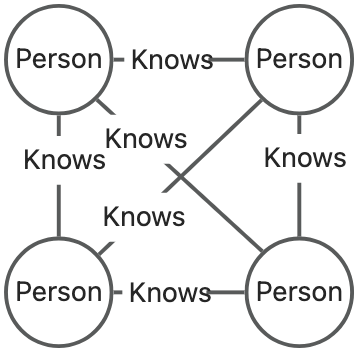
\includegraphics[width=.3\linewidth]{./figures/intro-pattern.png}
    \caption{Pattern graph corresponding to the conditions in the SQL query.}
    \label{fig:intro-pattern}
\end{figure}


Indeed, the conditions specified within this SQL statement collectively establish the structure of a pattern graph.
As shown in Fig.~\ref{fig:intro-pattern}, there are four vertices representing four persons, and these four persons form a complete graph.
Therefore, this SQL query can be expressed as a graph query.
The corresponding expression following the grammar of Cypher \cite{opencypher} is as follows: 
\begin{lstlisting}
    MATCH (p1:Person)-[:Knows]-(p2:Person)-[:Knows]-(p3:Person)-[:Knows]-(p4:Person),
        (p1)-[:Knows]-(p3), (p2)-[:Knows]-(p4)
    RETURN p1.id, p2.id, p3.id, p4.id;
\end{lstlisting} 
This graph query expression is much more concise and understandable than that in SQL.
It suggests that SQL is not always the optimal choice, and sometimes employing graph queries is more advantageous.
Then, in order to combine the extensive developments made in SQL queries over the years with the benefits of graph queries, it would be helpful for SQL to support both relational and graph queries.

Following this idea, the striking SQL/Property Graph Queries (abbr.~SQL/PGQ) is proposed.
In detail, SQL/PGQ is a part of SQL 2023 and its grammar allows to define and query graphs in SQL/PGQ expressions.
Consequently, some complex relational queries (such as those containing multiple joins) can be represented as relatively simple graph queries.
Specifically, graphs in SQL/PGQ are presented as views, and vertices and edges in the graphs are represented as tables.
It implies that with SQL/PGQ, graph queries and relational queries can be expressed in one statement and optimized together for a better execution plan.
An example of an SQL/PGQ query is provided in Example \ref{example:introduction:sqlpgq}.

\begin{example}
    \label{example:introduction:sqlpgq}
    Suppose three tables, i.e., \textbf{Person, Knows, Department}, are stored in the relational database.
    With SQL/PGQ, a graph view named \textbf{friendship\_graph} is created based on tables \textbf{Person} and \textbf{Knows}.
    Specifically, rows in table \textbf{Person} represent the vertices in the graph while rows in table \textbf{Knows} represent the edges.
    Besides, the department a person belonging to is stored in table \textbf{Person} as a foreign key (i.e., \textit{dept\_id}).

    Suppose we are going to find three persons satisfying: (1) They know each other; (2) Two of them belong to the Department of Computer Science.
    Then, the corresponding SQL/PGQ query is as follows:
    \begin{lstlisting}
        SELECT pn1, pn2, pn3
        FROM Department p, GRAPH_TABLE (friendship_graph
            MATCH (p1:Person)-[:Knows]-(p2:Person)-[:Knows]-(p3:Person),
            (p1)-[:Knows]-(p3)
            COLUMNS (
                p1.name as pn1,
                p1.dept_id as dept1,
                p2.name as pn2,
                p2.dept_id as dept2,
                p3.name as pn3,
                p3.dept_id as dept3)
        ) f
        WHERE dept1 = p.dept_id
        AND dept2 = p.dept_id AND
        AND p.dept_name = 'Computer Science';
    \end{lstlisting}
    According to the first condition, the obtained three persons should form a triangle.
    It is a problem of pattern matching, and such triangles are searched for on \textbf{friendship\_graph}.
    The output of the graph query is a table (named \textbf{f}) with six columns, i.e., pn1, dept1, pn2, dept2, pn3, and dept3, representing the names of the three persons and the identifiers of the departments they belonging to.

    For the second condition, due to the existence of the foreign key, it is efficient to perform natural join between table \textbf{f} and table \textbf{Department} to obtain the ideal results.
    Please note that the outputs of graph queries are still tables, and the outputs can be treated as tables within relational queries.
\end{example}

To support SQL/PGQ queries, it is more reasonable to enhance relational databases with the capability to process graph queries.
The reason is that relational databases have been widely utilized in both academia and industry, and it is costly and impractical to migrate data from relational databases to graph databases.
After the SQL/PGQ query is parsed, relational databases need to optimize the obtained abstract syntax tree (abbr.~AST).
However, since graph queries are allowed in SQL/PGQ queries, the existing relational databases can hardly optimize ASTs with graph operators.
Intuitively, there are some possible solutions, which can be mainly categorized into four types.
The stages of query optimization that these four types of solution are involved in respectively are shown in Fig.~\ref{fig:catagory}.

\begin{figure*}
    \centering
    \begin{subfigure}[b]{0.4\linewidth}
        \centering
        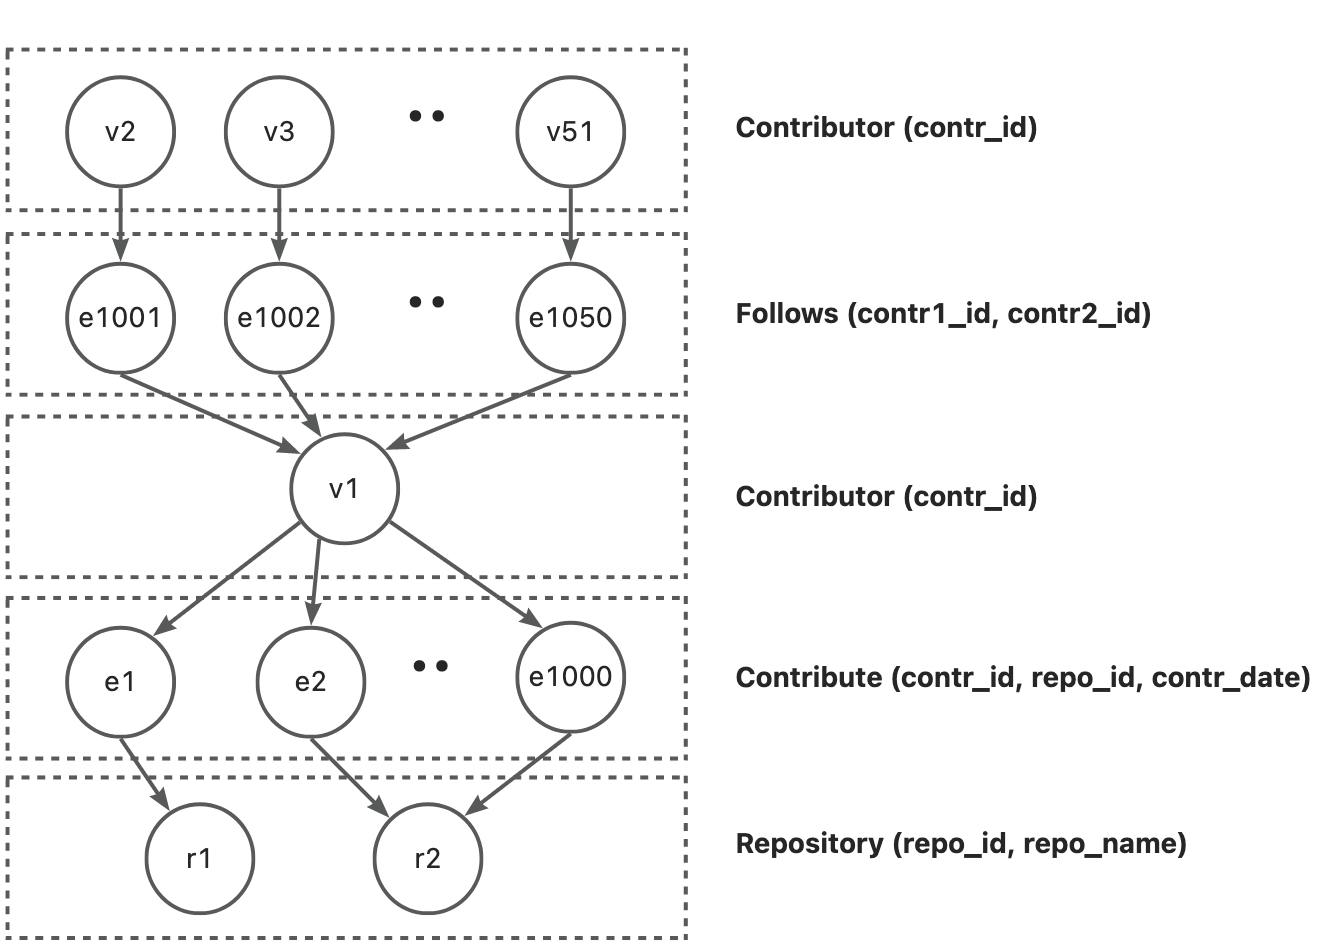
\includegraphics[width=\linewidth]{./figures/intro-order-case.png}
        \caption{Relationship 1.}
        \label{fig:intro-order-case}
    \end{subfigure}
    \begin{subfigure}[b]{0.4\linewidth}
        \centering
        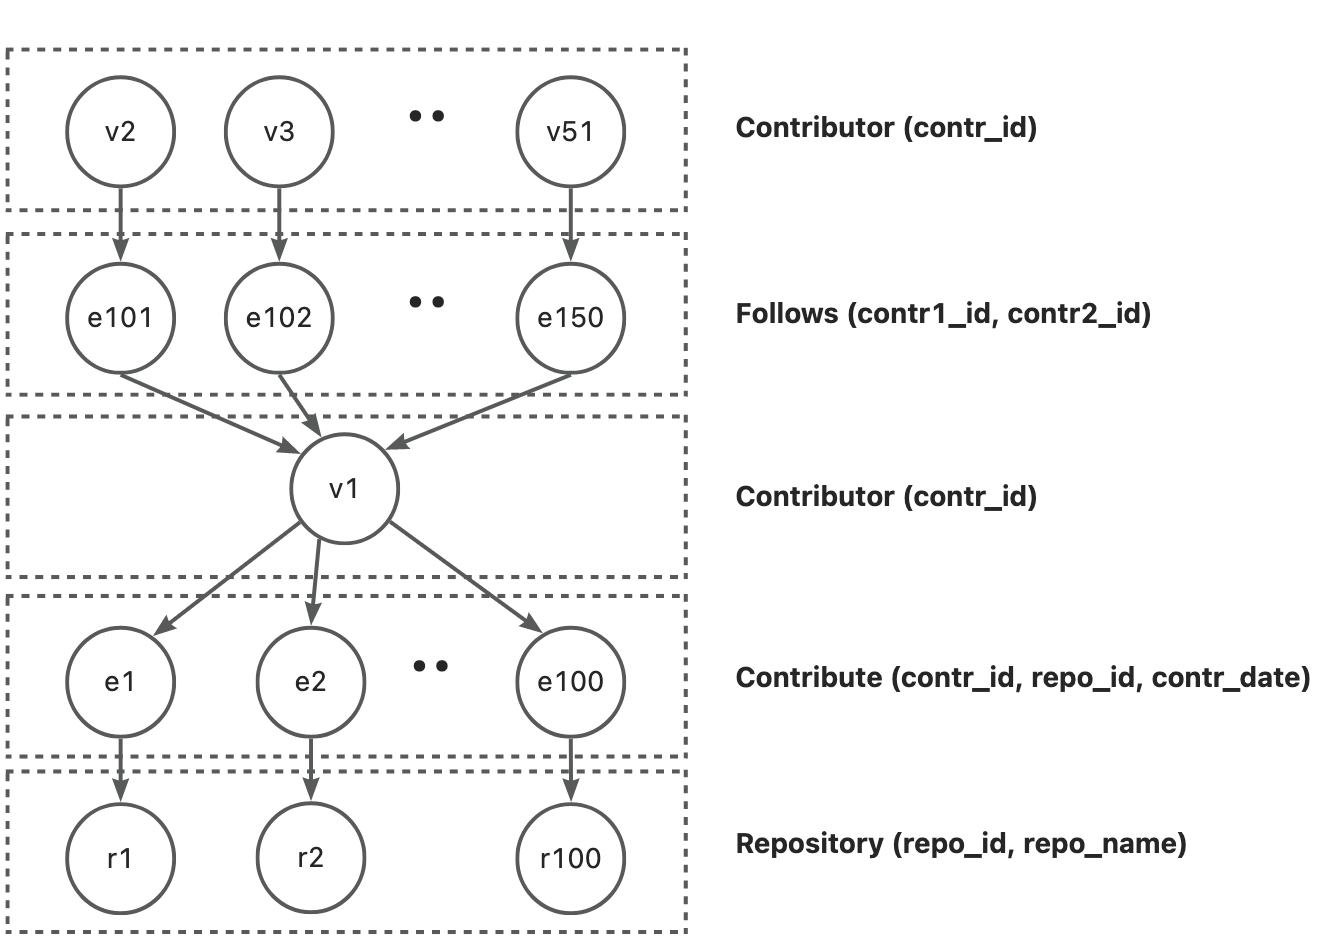
\includegraphics[width=\linewidth]{./figures/intro-order-case-2.png}
        \caption{Relationship 2.}
        \label{fig:intro-order-case2}
    \end{subfigure}
    \caption{Graphs representing the relationships among tuples in different tables. In detail, tuples in Tables \textbf{Contributor} and \textbf{Repository} represent vertices in the graph, while those in Tables \textbf{Follows} and \textbf{Contirbute} represent edges.}
    \label{fig:intro-replace-example}
\end{figure*}

\begin{figure*}
    \centering
    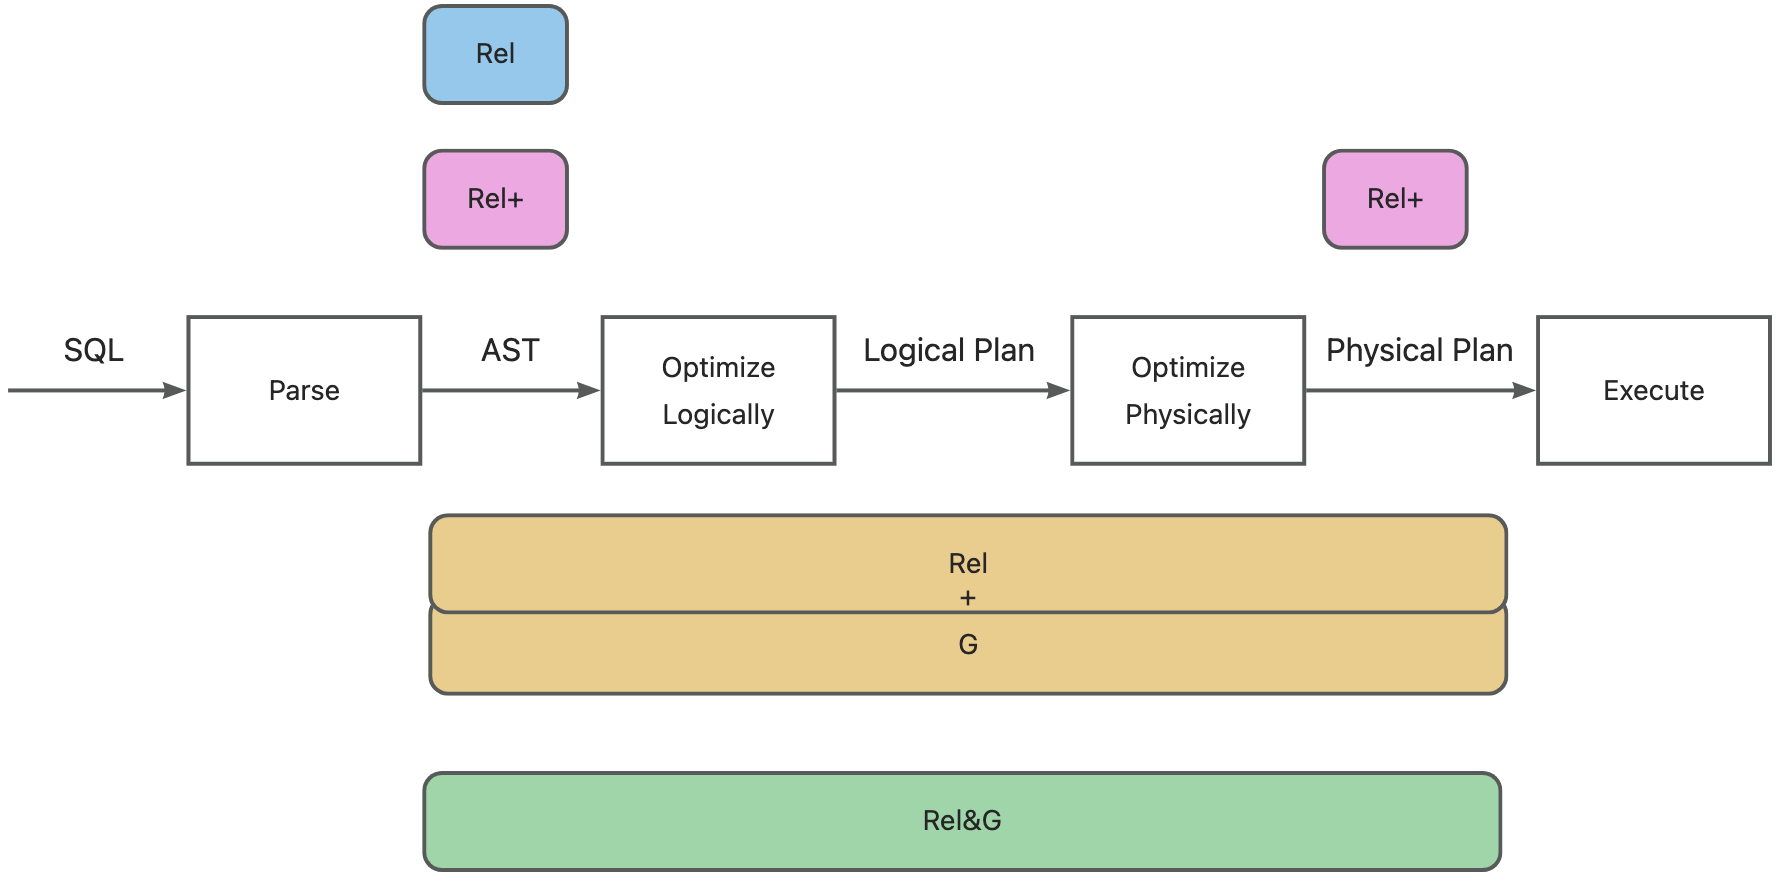
\includegraphics[width=.6\linewidth]{./figures/catagory.png}
    \caption{The stages of query optimization that the four kinds of solutions are involved in.}
    \label{fig:catagory}
\end{figure*}

\textbf{Solution 1 ($Rel$)}. 
The most direct solution is to transform graph queries to relational ones, and then optimize the new queries with relational optimizers.
Apache Age \cite{apache-age} is a typical example.
However, methods of this type only take effect in the stage of logical optimization and degrade into relational optimizers.
Therefore, they lose the chance of query optimization from the graph perspecitve.

\begin{example}
    Given four tables \textbf{Contributor}, \textbf{Follows}, \textbf{Contribute}, and \textbf{Repository} as shown in Fig.~\ref{fig:intro-order-case}, the relationships among their tuples are presented.
    Specifically, edge (v1, e1) means that e1.contr\_id = v1.contr\_id and edge (e1, r1) means that e1.repo\_id = r1.repo\_id.
    Moreover, suppose graph indices have been built on tables \textbf{Follows} and \textbf{Contribute}.
    Then, given a contributor, the followers of the contributor and the repositories the contributor contributes to can be directly retrieved with the indices, respectively.

    Suppose we are going to find the followers of $v1$, and the query is as follows:
    \begin{lstlisting}
        SELECT pid
        FROM GRAPH_TABLE (graph_view
            MATCH (p1:Contributor)-[:Follows]->(p2:Contributor {id: 1})
            COLUMNS (p1.id as pid)
        );
    \end{lstlisting}
    If the graph query is transformed to the corresponding relational query, then the followers of $v1$ can only be found with a join between \textbf{Contributor} and \textbf{Follows}, and another join between the resultant table and \textbf{Contributor}.
    In this process, the graph indices cannot be utilized, and the process is far from efficient.
\end{example}


\textbf{Solution 2 ($Rel^+$)}.
Methods of this type build graph indices on relational databases and introduce new operators to perform graph queries based on the indices.
However, these new operators are applied after the optimial physical plan is obtained with the relational optimizer.
As shown in Fig.~\ref{fig:catagory}, such methods are separately involved in the stages of logical optimization and physical optimization.
It means that the optimizations w.r.t.~graph operators at the logical layer and the physical layer are disjointed.
To be more specific, the cost of new operators introduced in physical optimization are unawared in logical optimization.

The optimizer in GrainDB \cite{graindb} is a representative of type $Rel^+$.
GrainDB builds RID indices on DuckDB \cite{duckdb}, and proposes two new join methods, i.e., sip-join and merge-sip-join.
In detail, sip-join gets adjacent edges of vertices or gets adjacent vertices of edges based on the RID indices, while merge-sip-join obtains the neighbors of vertices.
Since GrainDB follows the grammar of SQL, given a SQL/PGQ query, the query is transformed to the equal relational query frist, and then GrainDB optimizes the query with the relational optimizer of DuckDB to obtain the optimal execution plan.
Next, GrainDB replaces some hash-joins in the plan with sip-joins and merge-sip-joins to leverage the graph indices.
It indicates that the cost-based optimization in GrainDB only finds the optimal execution plan before the graph indices are awared.
Therefore, the plan can be suboptimal after replacement.
Moreover, some efficient replacement cannot be applied w.r.t.~the obtained execution plan due to the order of joining tables representing vertices and edges.
An example is shown as follows.

\begin{example}
    Given four tables as shown in Fig.~\ref{fig:intro-order-case}, a SQL/PGQ query is as follows:
    \begin{lstlisting}
        SELECT contr_id, repo_name 
        FROM GRAPH_TABLE (graph_view
            MATCH (p2:Contributor)-[f:Follows]->(p1:Contributor {contr_id: 1})-[c:Contribute]->(r:Repository)
            COLUMNS (p2.contr_id as contr_id,
                    r.repo_name as repo_name)
        );
    \end{lstlisting}
    %\begin{lstlisting}
    %    SELECT p2.contr_id, repo_name
    %    FROM Contributor p1, Follows f, Contributor p2, Contribute c, Repository p
    %    WHERE p1.contr_id = 1 
    %    AND p1.contr_id = f.contr2_id 
    %    AND p2.contr_id = f.contr1_id
    %    AND p1.contr_id = c.contr_id 
    %    AND c.repo_id = r.repo_id;
    %\end{lstlisting}
    From the perspecitve of a relational database (e.g., DuckDB), the best join order can be \textbf{p1$\rightarrow$f$\rightarrow$p2$\rightarrow$c$\rightarrow$r}, since tables \textbf{Follows} and \textbf{Contributor} have much smaller cardinalities than table \textbf{Contribute}.
    Then, by replacing the join operators with getNeighbor, the finally obtained execution plan is \textbf{p1$\xrightarrow{\textit{getNeighbor}}$p2$\xrightarrow{\textit{getNeighbor}}$r}.

    However, as $v_1$ has much fewer neighbors in table \textbf{Repository} than in table \textbf{Contributor}, join order \textbf{p1$\xrightarrow{\textit{getNeighbor}}$r$\xrightarrow{\textit{getNeighbor}}$p2} would be more efficient from the perspective of graph databases.
    Therefore, it suggests that 
    replacing relational operators with graph operators after optimization with relational optimizers can miss optimial execution plans.

    Besides, given the relationships among the tuples as shown in Fig.~\ref{fig:intro-order-case2}, the best join order from the perspective of a relational database like DuckDB can be \textbf{p1$\rightarrow$f$\rightarrow$c$\rightarrow$p2$\rightarrow$r}.
    Then, \textbf{p1$\rightarrow$f} and \textbf{c$\rightarrow$p2} cannot be replaced with \textbf{p1$\xrightarrow{\textit{getNeighbor}}$p2} and some efficient execution plans are missing.

    %An example about replace join with getV/getE/getNeighbor,
    %or the example of duckdb, whether to indicate more constraints (due to the unawareness of getNeighbor)
\end{example}


\textbf{Solution 3 ($Rel+G$)}.
According to the grammar of SQL/PGQ, the graph queries usually starts with keyword GRAPH\_TABLE.
Therefore, graph queries can be easily distinguished in SQL/PGQ queries.
Hence, it is possible to optimize graph queries first with graph optimizers, and then optimize the relational query with relational optimizers.
As shown in Fig.~\ref{fig:catagory}, the logical and physical optimization are related, and the cost of graph operators are estimated in the process of optimization.
However, this solution still has limitations, e.g., graph queries and relational queries are optimized separately, and cross-queries optimizations are missing.
An example about this limitation is presented.

\begin{example}
    \label{example:push_down}
    Suppose we are going to find persons that know John and the query expression is as follows:
    \begin{lstlisting}
        SELECT p FROM GRAPH_TABLE (friendship_graph 
            MATCH (p1:Person)-[:Knows]-(p2:Person)
            COLUMNS (p1.name as p, p2.name as p2)
        )
        WHERE p2 = 'John';
    \end{lstlisting}
    For $Rel+G$ methods, the graph query is first optimized with a graph optimizer, and the optimized plan finds all pairs of persons that know each other.
    Then, the relational optimizer optimizes the relational query, which finds the persons that know John.
    Please note that the condition ``p2 = 'John''' in the relational query can be pushed down into the graph query, so that the graph query only returns persons that know John.
    The optimized query is as follows.
    \begin{lstlisting}
        SELECT p FROM GRAPH_TABLE (friendship_graph 
            MATCH (p1:Person)-[:Knows]-(p2:Person {name: 'John'})
            COLUMNS (p1.name as p)
        );
    \end{lstlisting}
    However, since $Rel+G$ methods optimize relational queries and graph queries separately and do not apply cross-queries optimizations, the condition cannot be pushed down and the optimal execution plan is missed.
\end{example}

In this paper, we propose \textbf{Solution 4 ($Rel\&G$)}, which optimizes the graph queries and relational queries simultaneously with cross-queries optimizations.
Such a solution can fully leverage the advantages of both relational optimizers and graph optimizers.
In detail, we propose a new converged optimization framework of this type for SQL/PGQ.
The framework first generates the converged logical plan consisting of a relational subplan and several graph subplans.
Then, optimization strategies including CBOs and RBOs are applied to optimize inside and crossing subplans.
The contributions of this paper are mainly as follows:

(1) To the best of our knowledge, this is the first optimization framework for SQL/PGQ query optimization.
Property graphs are represented as views in SQL/PGQ, and vertices and edges are associated with tables in the relational databases.
Then, it is crucial to offer a converged query optimizer efficient for SQL/PGQ queries to optimize both relational and graph queries in SQL/PGQ statements.

(2) The framework proposes a new Scan operator named ScanGraphTable to retrieve data from graph tables obtained with graph queries.
The output of ScanGraphTable is a relational table and it bridges the gap between graph subplans and relational subplans.

(3) We prove that graph pattern matching expressed in graph queries of SQL/PGQ can be expressed with graph relational algebra, which confirms that the converged graph relational optimization framework can optimize SQL/PGQ queries and obtain correct results.


% In the framework, we design and implement numerous important operators for graph optimizer, including getV, getE, getNeighbor, and extendIntersect.
% Specifically, the extendIntersect operator is helpful in supporting worst-case optimality.

(4) Theoretical analysis on the complexity of the optimization framework is conducted.
The obtained theorems prove that for graph queries, the join order optimization with a graph optimizer can be exponentially faster than that with a relational optimizer. 
It theoretically confirms that relational optimizer is usually not suitable for graph queries, and it is indispensable for the existence of a converged optimization framework.

(5) Extensive experiments are conducted to show the efficiency of the proposed converged query optimization framework.
The experimental results show that the framework can be ?$\times$ faster than the baselines.

The rest of this paper is organized as follows.


The existing methods for optimizing the SPJM queries can be divided into four categories.
The main difference between these methods lies in the approach to handling the matching operator.
Before the details of these methods are introduced, concepts about graph structure and graph matching decomposition are proposed as follows.

\subsection{Graph Structure}

The definition of graph structure is as follows.

\begin{definition}[Graph Structure, abbr.~GS]
    Graph structure refers to the connectivity relationships between vertices and edges within the graph, which can be stored in graph indices in varied data structure such as adjacent lists.
\end{definition}

With graph structure, tables can be joined more efficiently.
For example, when two tables representing persons and friendships respectively are joined together, the rows that can be joined are quickly located using graph indices.
Therefore, when graph indices are available, using join methods that can leverage graph indices is a more efficient choice.

\subsection{Graph Matching Decomposition}

Given a matching operator, it can be decomposed into two new matching operators.
By joining the results of the new matching operators, the results of the original matching operator can be obtained.
Decomposing the matching operator recursively can result in a tree, which is called the match scanning plan.
Each tree node represents an operator.
\textbf{Without loss of generality, suppose for each join operator, the left subtree is computed first}.
For each internal node, it can represent the join, selection, or projection operator.
Take the join operator as an example.
Internal nodes representing join operators are generated when matching operators are decomposed.
Suppose a matching operator $TN_0 = \mathcal{M}(V, E, \mathcal{P}_0)$ is decomposed into two child operators, i.e., $TN_1 = \mathcal{M}(V, E, \mathcal{P}_1)$ and $TN_2 = \mathcal{M}(V, E, \mathcal{P}_2)$.
Denote the sets of vertices and edges in a pattern $\mathcal{P}$ by $\mathcal{P}.V$ and $\mathcal{P}.E$, respectively.
Then, we have $\mathcal{P}_0.V = \mathcal{P}_1.V \cup \mathcal{P}_2.V$, $\mathcal{P}_0.E = \mathcal{P}_1.E \cup \mathcal{P}_2.E$, $\mathcal{P}_1.V \cap \mathcal{P}_2.V \neq \emptyset$, and $\mathcal{P}_1.E \cap \mathcal{P}_2.E = \emptyset$.
After $TN_0$ is decomposed, it is transformed to an internal node representing the join operator, and $TN_1$ as well as $TN_2$ are its child nodes.


Each leaf node is a minimum matching component, and the definition is as follows.

\begin{definition}[Minimum Matching Component]
    A matching operator is called a minimum matching component iff the matching of the pattern has a specific physical implementation according to the optimizer and the matching operator will not be further decomposed.
\end{definition}

In the process of decomposing the matching operator, an important point is the order in which the nodes and edges are decomposed each time.
In other words, it is necessary to determine the order of the joins to generate the pattern specified in the original matching operator.
Therefore, optimizers are applied to optimize the order.

For relational optimizers, the minimum matching components are matching operators whose patterns only contain a vertex or an edge.
Then, the physical implementation of such matching operators is scanning the tables of the corresponding vertices or edges, respectively.
Therefore, for relational optimizers, the matching operator will be replaced with selection operators, projection operators, and a sequence of join operators between tables representing vertices and edges.

For graph optimizers, the minimum matching components are more diverse.
Following the idea of StarJoin \cite{}, matching operators whose patterns consist of a vertex, an edge, or a complete star are considered as minimum matching components.
Here, the pattern consisting of an edge actually contains the edge and its adjacent two vertices.
Let $TL = \mathcal{M}(V, E, \mathcal{P})$ be a minimum matching component, which is also a leaf node of the tree, and $\mathcal{P}$ is a complete star.
Also, denote the parent node of $TL$ by $Join_{TL}$.
A complete star is a tree of depth one with at least three vertices, whose root is called the core, while the other nodes are called the outsiders.
For each outsider $v_o$ of a complete star, $v_o$ should exist in the pattern of matching operators in $Join_{TL}$'s left subtree.
Besides, $TL$ should be in the right subtree of $Join_{TL}$.

If graph strucutre is utilized, the minimum matching component whose pattern is an edge can be implemented with joins that leverage graph indices, and the neighbors of vertices can be obtained efficiently.
If graph structure is not utilized, such a pattern is obtained by two joins between tables representing vertices and edges.

For the minimum matching component $\mathcal{MMC}$ whose pattern is a complete star, it can be implemented with a table scan of the core.
The outsiders are not handled, because they are already computed in the left subtree of the parent node of $\mathcal{MMC}$.
$\mathcal{MMC}$'s parent node representing the join operator is then implemented with extend-intersection.
Specifically, in the process of extend-intersection, the neighbors of the outsiders are obtained by joining them with tables representing edges and the results of $\mathcal{MMC}$, respectively.
The common neighbors are obtained by calculating the intersection.
Please note that if graph structure is available, the neighbors can be obtained with graph indices.
With extend-intersection, the times of joins are reduced significantly, and it has better performances than joining tables one by one.


Moreover, for optimizers, cost of different join orders should be estimated.
Normally, the cardinalities of tables are utilized, which are low-order statistics of the patterns.
Since the patterns in matching operators are graphs, it is more efficient to estimate the cost with graph statistics.

\begin{definition}[Graph Statistics]
    Graph statistics record the occurrence of structures within the graph, such as the number of triangles appearing in the graph.
\end{definition}

Specifically, graph statistics can reflect the higher-order features of graphs (e.g., the number of subgraphs), and well represent the characteristics of graphs.
Thus, with garph statistics, better join orders with lower cost can be obtained.

The aforementioned optimizations are collectively referred to as optimizations based on graph matching decompostion (abbr.~GMD).


\subsection{Existing Methods}

The general approach to handling the SPJM queries is to first transform it into an SPJ queries, and then optimize the SPJ queries to obtain the corresponding physical plans.
It is proved in Theorem \ref{theorem:spjm-to-spj} that SPJM queries can always be losslessly converted to SPJ queries.
Existing methods can be divided into four categories based on whether GS and GMD are utilized in the process.

(1) \emph{SPJM $\rightarrow$ SPJ $\rightarrow$ Physical Plan}.
This type of method does not apply GS and GMD in the process of optimizing the SPJM queries.
In detail, matching operators are decomposed into minimum matching components, whose patterns contain only a vertex or an edge.
Such matching operators are converted to table scans, and a new SPJ query is generated and optimized.
This type of method degrades into relational optimizers and loses the chance of query optimization from the graph perspective.
An typical method of this type is Apache Age.


In order to leverage the graph information to obtain better physical plans, the second kind of method is proposed.

(2) \emph{SPJM $\rightarrow$ SPJ $\xrightarrow{GS}$ Physical Plan}.

For this type of method, graph structure is utilized in the process of optimizing the SPJ queries.
Specifically, with graph indices, the connectivity between vertices and edges can be obtained efficiently.
Therefore, new physical implementations of joins can be constructed to leverage the benefits of graph indices.

The optimizer in GrainDB is a representative of this type.
GrainDB builds RID indices on DuckDB \cite{duckdb}, and proposes two new join methods, i.e., sip-join and merge-sip-join.
In detail, sip-join gets adjacent edges of vertices or gets adjacent vertices of edges based on the RID indices, while merge-sip-join obtains the neighbors of vertices.
Given a SPJM query, it is first transformed to the equal SPJ query, and then GrainDB optimizes the query with the relational optimizer of DuckDB to obtain the optimal execution plan.
Next, GrainDB replaces some hash-joins in the plan with sip-joins and merge-sip-joins to leverage graph indices.

It indicates that the cost-based optimization in GrainDB only finds the optimal execution plan before the graph indices are awared.
Therefore, the plan can be suboptimal after replacement.
Moreover, some efficient replacement cannot be applied w.r.t.~the obtained execution plan due to the order of joining tables representing vertices and edges.


It is also reasonable to exploit the capability of graph matching decomposition for better optimization.
Then, the third kind of method is proposed as follows.

(3) \emph{SPJM $\xrightarrow{GMD}$ SPJ $\rightarrow$ Physical Plan}.

This type of method convert SPJM queries to SPJ queries in a different manner.
Specifically, graph matching decomposition is applied and the matching of complete stars is a minimum matching component.
With GMD, higher-order features of graphs are leveraged, and cost of join orders can be estimated more accurately.
Please note graph structure is not applied in this type of method.
Thus, when we optimize SPJ queries and generate physical plans, the physical implementations of joins cannot utilize the graph indices, including the implementation of extend-intersection.


(4) \emph{SPJM $\xrightarrow{GMD}$ SPJ $\xrightarrow{GS}$ Physical Plan}.

This is the method utilized in this paper.
Compared to method (3), this kind of methods further utilize graph strucutre in optimization.
Therefore, physical implementations of join operators can utilize the graph indices and the common neighbors can be obtained more efficiently in extend-intersection.
Besides, in the process of graph matching decomposition, since the higher-order statistics are utilized (i.e., the number of subgraphs), the cost of joins are estimated assuming that graph indices can be utilized in execution.
Therefore, cost estimation is more accurate for when graph indices are applicable. 

\subsection{Proof}

\begin{theorem}
    \label{theorem:spjm-to-spj}
    The SPJM query can be losslessly converted to an SPJ query.
\end{theorem}
\begin{proof}
    Clearly, if the matching operator can be expressed with selection, projection, and join operators (abbr.~SPJ operators), then naturally, the theorem is correct.
    We begin with matching operators with homomorphic semantics, and prove the theorem using induction.
    In this proof, vertices and edges are elements in a pattern and a pattern $\mathcal{P}$ is called a strict pattern, if the adjacent vertices of each edge in $\mathcal{P}$ are specified in the pattern (e.g., (u)-[e]-(v)).
    Otherwise, the pattern is called a loose pattern (e.g., (u)-[e]).
    Without the loss of generality, matching operator $\mathcal{M}(V, E, \mathcal{P})$ is considered.
    Then, induction is conducted on the number of elements in $\mathcal{P}$.
    
    When there is only one element in $\mathcal{P}$ (e.g., $\mathcal{P}=(u:\text{Person})$), such a pattern can be expressed with the selection operators (e.g., $\sigma_{label=\text{``Person''}}(V)$).
    Please note that is there are more constraints on the element (e.g., the returned person should be at least 18 years old), more constraints can be specified with the selection operators.

    Suppose for patterns with at most $n$ elements, they can be expressed with SPJ operators.
    Denote the sequence of SPJ operators that have the same meaning as pattern $\mathcal{P}$ by $\mathcal{E}_{\mathcal{P}}$.
    When there are $n+1$ elements in a pattern $\mathcal{P}$, let $v$ be a vertex in $\mathcal{P}$, and $e_1, \cdots, e_k$ are the edges connecting $v$ with the other vertices in $\mathcal{P}$.
    $\widehat{\mathcal{P}}$ is the strict pattern obtained by removing $v$ and $e_1, \cdots, e_k$ from $\mathcal{P}$.
    Then, $\mathcal{P}$ can be expressed with SPJ operators as follows:
    \begin{equation*}
        \mathcal{E}_{\widehat{\mathcal{P}}} \Join \sigma_{label=el_1}(E) \Join \cdots \Join \sigma_{label=el_k}(E) \Join \sigma_{label=vl}(V),
    \end{equation*}
    where $vl$ is the label of $v$, $el_1, \cdots, el_k$ are labels of $e_1, \cdots, e_k$.
    In conclusion, adopting the homomorphism semantics, the matching operator can be expressed with SPJ operators.

    Furthermore, when the matching operator adopt other semantics (e.g., isomorphism), it is straightforward to add some constraints on the elements with selection operators.
    For instance, when the isomorphism semantics is adopted, constraints should be added to ensure that different vertices in the pattern graph match with different vertices in the database.
    Therefore, the theorem is correct. 
\end{proof}